\documentclass[a4paper,11pt]{article}
\usepackage[margin=25mm]{geometry}
\usepackage{fontspec}
\usepackage{graphicx}
\usepackage[hidelinks,breaklinks=true]{hyperref}
\urlstyle{same}
\IfFontExistsTF{Noto Serif CJK TC}{\setmainfont{Noto Serif CJK TC}}{%
  \IfFontExistsTF{PMingLiU}{\setmainfont{PMingLiU}}{\setmainfont{PingFang TC}}}
\XeTeXlinebreaklocale "zh"
\XeTeXlinebreakskip=0pt plus 0.5pt
\setlength{\parindent}{0pt}
\setlength{\parskip}{4pt plus 1pt}
\setlength{\emergencystretch}{3em}
\renewcommand{\baselinestretch}{1.27}
\setcounter{secnumdepth}{0}
\makeatletter
\renewcommand{\section}{\@startsection{section}{1}{0pt}
  {1.05\baselineskip plus .2\baselineskip}{.32\baselineskip}
  {\normalfont\large\bfseries}}
\makeatother
\raggedbottom
\begin{document}
{\noindent\fontsize{22}{30}\selectfont\bfseries 引文定位資訊與原文回查時間\par}
{\small 稿證教學範例　｜　教學示例，數值為模擬資料\par}
\vspace{0.35em}
{\bfseries 摘要}\par
筆記多記一個頁碼或小節，回頭找原句時會差多少時間？本例為六條引文各設計兩種筆記，一種僅記書目，另一種加記原文位置。每條引文在兩種條件下各有一筆模擬時間，計時單位為秒。「僅記書目」共 6 筆，回查時間平均為 78 秒。「加記原文位置」共 6 筆，回查時間平均為 38 秒。這組秒數是為示範程式而設定的。要評估研究者實際能省下多少時間，得另行招募讀者，記錄他們回查原句的過程。
\par{\small 關鍵詞　引文查核、研究筆記、資料溯源}\par
\section{研究問題}

修稿時，書目通常還在，真正難找的是當初據以寫下判斷的那一句。若筆記只留下篇名，作者得再讀一次原文。把頁碼或小節一起記下，查找的路徑便有了較明確的起點。

\section{相關文獻}

Sandve 等人建議，研究者應留下足以說明每項結果如何產生的紀錄。本文借用這項原則檢視引文筆記。另一位讀者拿到筆記後，找得到當初支持這句話的材料嗎？\footnote{Geir Kjetil Sandve et al., “Ten Simple Rules for Reproducible Computational Research,” PLOS Computational Biology 9, no. 10 (2013): e1003285，Rule 1。 \href{https://doi.org/10.1371/journal.pcbi.1003285}{https://doi.org/10.1371/journal.pcbi.1003285}}

世界資訊網協會的 PROV 資料模型區分實體、活動及衍生關係。依這個區分，原文和筆記可以分別登錄，再說明筆記如何取材自原文。這套模型能指引資料欄位的設計，回查耗時仍須另外測量。\footnote{Luc Moreau and Paolo Missier, eds., PROV-DM: The PROV Data Model (W3C, April 30, 2013)，第 2.1.1 節及第 2.1.2 節。 \href{https://www.w3.org/TR/2013/REC-prov-dm-20130430/}{https://www.w3.org/TR/2013/REC-prov-dm-20130430/}}

\section{研究方法}

本例為六條引文各設計兩種筆記，一種僅記書目，另一種加記原文位置。每條引文在兩種條件下各有一筆模擬時間，計時單位為秒。

這裡把「找到引用的原句」定為計時終點。查到原句後，仍要讀上下文，判斷引文能否支持正文的說法。這段判讀所花的時間，另屬一個研究問題。

\begin{center}\begin{minipage}{0.94\linewidth}\centering
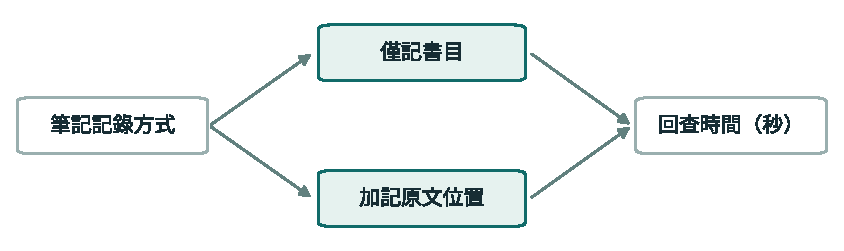
\includegraphics[width=0.86\linewidth]{figures/concept.pdf}
\par\small\bfseries 圖 1　比較條件與觀察指標
\par\normalfont\footnotesize 資料來源　project.json 與 measurements.csv。箭線連結比較條件及觀察指標。
\end{minipage}\end{center}

\section{研究結果}

「僅記書目」共 6 筆，回查時間平均為 78 秒。「加記原文位置」共 6 筆，回查時間平均為 38 秒。

第 4 條引文值得單獨看。模擬紀錄裡，僅記書目時花了 42 秒，加記位置時花了 46 秒。即使兩組平均有差，回到個別引文，順序也可能倒過來。

\begin{center}\begin{minipage}{0.94\linewidth}\centering
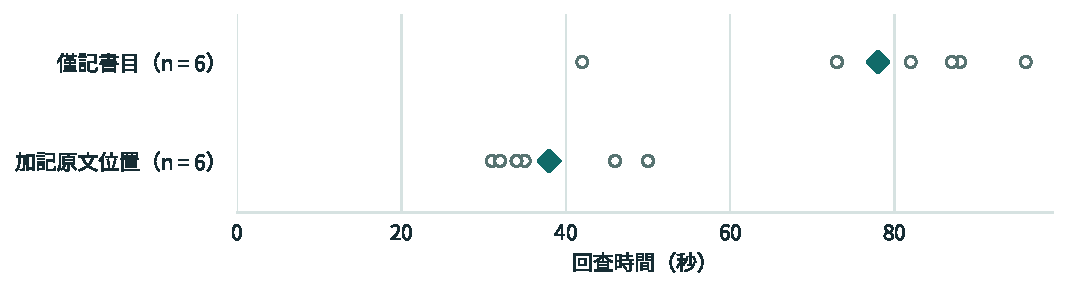
\includegraphics[width=0.86\linewidth]{figures/values.pdf}
\par\small\bfseries 圖 2　各組回查時間的分布
\par\normalfont\footnotesize 資料來源　measurements.csv。圓點代表單筆紀錄，菱形代表各組平均。
\end{minipage}\end{center}

\section{討論與限制}

這組秒數是為示範程式而設定的。要評估研究者實際能省下多少時間，得另行招募讀者，記錄他們回查原句的過程。

正式施測時，同一個人第二次看到相同引文，可能已經記得原句的位置。可把引文分成兩組，交錯安排兩種筆記的使用順序，再比較結果。
\section{參考文獻}
\begingroup\small\raggedright
Moreau, Luc, and Paolo Missier, eds. PROV-DM: The PROV Data Model. W3C Recommendation, April 30, 2013. \href{https://www.w3.org/TR/2013/REC-prov-dm-20130430/}{https://www.w3.org/TR/2013/REC-prov-dm-20130430/}\par
Sandve, Geir Kjetil, Anton Nekrutenko, James Taylor, and Eivind Hovig. “Ten Simple Rules for Reproducible Computational Research.” PLOS Computational Biology 9, no. 10 (2013): e1003285. \href{https://doi.org/10.1371/journal.pcbi.1003285}{https://doi.org/10.1371/journal.pcbi.1003285}\par
\endgroup
\end{document}
